\chapter{调试通道总体设计与关键技术}

\section{总体设计}
	VxWorks的集成开发调试环境为Tornado,它使用串口和网口结合的方式来对目标机进行控制和数据传输,而目前对于大多数的设备而言都已经抛弃了串口,很多用于军事上的嵌入式设备都是专用设备,没有联网的需求,并不会配备网口,但是对于设备上产生的各种调试信息、日志信息都需要传输到我们的windows PC上来进行一个事后分析工作,因此我们需要设计一个新的调试通道来满足这些信息的传输要求,我们本次设计一个基于USB口转串口的底层驱动来实现该调试通道。
	调试通道的总体结构如\autoref{fig:debug-system-diagram}所示。
\begin{figure}[!h]
\centering
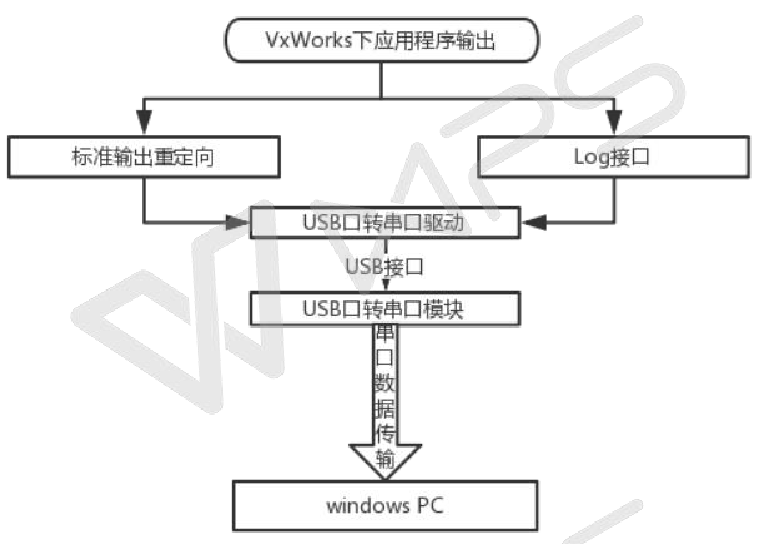
\includegraphics[width=.9\textwidth]{./graphics/debug-system-diagram.pdf}
\caption{调试通道整体结构图}\label{fig:debug-system-diagram}
\end{figure}
	
	整个调试通道主要分为两个模块:应用层的接口模块、USB口转串口模块。
	
	提供给应用层的接口模块负责将系统应用层的输出通过我们的USB口转串口驱动程序传输到windows PC机,输出的形式包括特定内容的格式化的输出和普通的重定向的输出,格式化的输出我们会使用自定义的Log接口进行格式控制,为此我们设计了一个自定义的Log协议格式,其中的内容包含有调试级别、调试信息所在的文件、调试信息所处的行号、输出该条调试信息的时间等;重定向的输出包括RTP模式下的重定向和task模式下的重定向,VxWorks中对于这两种模式需要使用不同的重定向方式。
	
	USB口转串口模块用于在VxWorks上实现一个USB口转串口驱动程序,负责将上层应用的信息传输到windows PC,包括一个特定需求的驱动程序一个普通的驱动程序。特殊需求的驱动程序相对于普通的驱动程序在流程和结构上进行了修改,以使其达到要求,具体的实现我们会在第三节进行介绍。两种实现方式中都会包含有驱动程序加载、卸载模块,设备的打开、关闭、读、写、控制模块。同时在驱动程序中还需要一个数据的管理模块,我们会使用循环缓冲区来管理数据。


\section{关键技术}

\subsection{VxWorks驱动开发}
	
	在VxWorks当中使用I/O子系统来管理设备驱动,I/O 子系统在整个VxWorks当中起着承上启下的作用,各种类型的设备都必须要向I/O子系统进行注册才能够被内核访问/cite{VxWorks内核解读}\cite{曹桂平2011VxWorks}。I/O子系统负责维护设备驱动中三个非常重要的数据结构:系统设备表、系统驱动表、系统文件描述符表,设备驱动程序初始化时会对硬件完成初始化的配置,同时会向I/O子系统注册自己,注册之后I/O子系统才能找到该驱动。我们从VxWorks 下的 I/O 系统和驱动程序的关系入手,分析 VxWorks 下 I/O 系统调用和驱动程序的实现过程,在VxWorks中设备驱动的访问过程如下:
\begin{enumerate}
\item 调用open()函数打开一个设备(假设设备名为/ttyUsb),I/O 系统会在系统的设备表中寻找这个名为/ttyUsb的设备项,并找到相应的驱动号; 
\item I/O系统在文件描述符当中保留一个文件描述符,然后在系统的设备驱动表中找到该设备注册的设备打开函数,调用这个函数,并返回设备描述符的指针;
\item I/O系统将设备描述符的指针存储在文件描述符列表的Device ID中,同时将对应的设备驱动号存储在文件描述符的Driver Num项。最后I/O系统返回该描述符的索引(即fd);
\item 应用程序当中使用这个fd来调用read()、write()函数。系统会根据fd自动找到相应的设备驱动号,进而找到相应的驱动例程\cite{解月江2004VxWorks设备驱动技术研究}。 
\end{enumerate}

\subsubsection{VxWorks I/O 系统}
	通常操作系统为了平台的无关性都会为应用程序提供一套标准的接口,VxWorks也不例外,它为应用层的提供了接口函数creat()、open()、unlink()、remove()、close()、rename()、read()、write()、ioctl()、lseek()、readv()、writev()等\cite{陈洋2007VxWorks}\cite{Wu2008Implementation}\cite{Zhang2010Design},我们将其称作为标准I/O 库。
	这样就可以通过调整底层驱动或者是接近驱动那部分的操作系统中间层来实现应用程序的通用性,提高应用层的开发效率,避免重复编码。在Mac OS、Linux、或Windows当中会把这套接口以标准库的形式呈现,但是在VxWorks中它们是由系统的内核实现的,都位于ioLib.c文件下。VxWorks与通用操作系统有很大的一个不同点是:VxWorks不区分用户态和内核态,用户层可以直接对内核函数进行调用,而无需使用陷阱指令之类的机制,以及存在使用权限上的限制。因此VxWorks提供给应用层的接口无需通过外围库的方式,而是直接以内核文件的形式提供\cite{VxWorks内核解读}。对于一般的设备而言,remove()接口是不需要实现的,I/O调用结构如\autoref{fig:I/O调用}所示。
	\begin{figure}[!h]
\centering
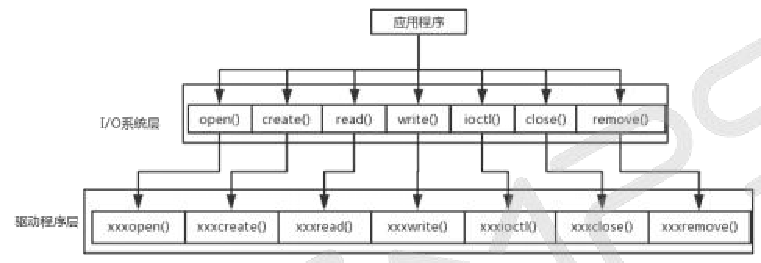
\includegraphics[width=1.0\textwidth]{./graphics/IOCall.pdf}
\caption{I/O调用}\label{fig:I/O调用}
\end{figure}

	
\subsubsection{系统设备表}
	系统设备表是VxWorks中为了管理系统上的所有设备而使用的一个链表。系统设备表在系统中的连接方式如\autoref{fig:VxWorks系统设备示意图}所示。wind内核规定每一个设备都必须使用一个DEV\_ HDR的结构来表示该设备,其定义如下\cite{VxWorks内核解读}:
\lstset{language=C}
\begin{lstlisting}
/*h/iosLib.h*/
typedef struct
{ 
  DL_NODE node; /* 设备链表节点 */ 
  short drvNum; /* 设备的驱动号 */ 
  char * name;/* 指向设备名 */ 
}DEV_HDR; /* 这个结构是所有设备自定义结构体的第一个成员 */
\end{lstlisting}
VxWorks系统提供了一个设备的注册函数iosDevAdd( DEV\_ HDR *pDevHdr, char *name, int drvnum)来将设备添加到系统设备表当中,系统设备表在每次添加设备时就会增加一个节点,删除设备时就会减少一个节点,它会为open()、close()、remove()这三个函数提供文件与设备的连接,当应用程序执行这三个函数中的一个时,IO系统会通过文件名对设备链表中的项进行匹配\cite{刘小军2008基于},VxWorks中使用最佳匹配的方式进行设备名匹配,匹配成功之后就使用这个设备驱动进行其他的文件操作。


\begin{figure}[!h]
\centering
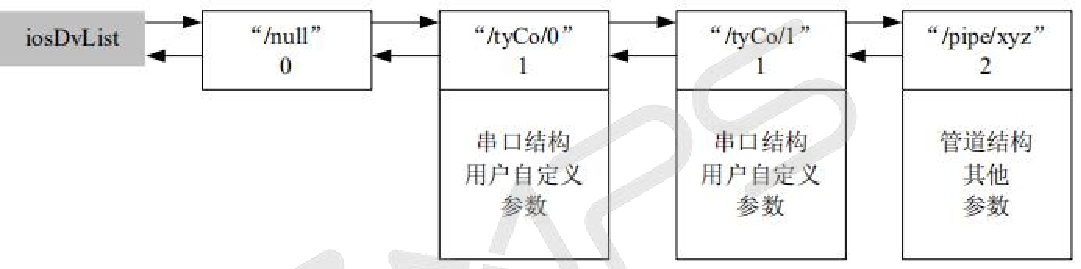
\includegraphics[width=1.0\textwidth]{./graphics/vxworks-device-link.pdf}
\caption{VxWorks系统设备示意图}\label{fig:VxWorks系统设备示意图}
\end{figure}

\subsubsection{系统驱动表}	
	系统驱动表用于管理当前注册到I/O子系统下的所有驱动程序,这些驱动可以是直接驱动硬件工作的驱动层,如一般的字符驱动,也可以是驱动中间层,如文件系统中间层,TTY 中间层,USB IO 中间层等。对于中间层驱动,下层硬件驱动将由这些中间层自身负责管理,而不再通过 IO 子系统。如串口底层驱动将通过 TTY 中间层进行管理,而不再通过IO子系统\cite{VxWorks内核解读}\cite{罗国庆2003VxWorks}。
	
	VxWorks中使用数组来实现系统驱动表,表中的每一个表项都是一个 DRV\_ ENTRY 类型的结构,该结构定义在 h/private/iosLibP.h文件当中,其定义如下\cite{VxWorks内核解读}:
\lstset{language=C}
\begin{lstlisting}
typedef struct  
{ 
  FUNCPTR de_create; /* 指向驱动的create()函数 */
  FUNCPTR de_delete; /* 指向驱动的delete()函数 */
  FUNCPTR de_open; 	 /* 指向驱动的open()函数 */
  FUNCPTR de_close;  /* 指向驱动的close()函数 */
  FUNCPTR de_read;   /* 指向驱动的read()函数 */
  FUNCPTR de_write;  /* 指向驱动的write()函数 */
  FUNCPTR de_ioctl;  /* 指向驱动的ioctl()函数 */
  BOOL de_inuse;     /* 用于指示表项是否空闲*/
} DRV_ENTRY;/* 系统驱动表中的条目 */ 
\end{lstlisting}
DEV\_ ENTRY结构体类型实际上就是一个函数指针结构,结构中每个成员都指向一个完成特定功能的函数,这些函数与用户层提供标准函数接口一一对应\cite{VxWorks内核解读}\cite{VxWorksDriverAPI}\cite{Wind2003VxWorks}。若成员 de\_ inuse 空闲则表示该表项未被使用。这个结构体中的函数指针实际指向的内容由驱动调用iosDrvInstall()函数来提供。 该函数的作用就是将驱动注册到系统驱动表当中,并根据注册的内容来填充DRV\_ ENTRY表项的内容。


\subsubsection{系统文件描述符表}
	系统描述符表用于管理当前系统打开的所有文件描述符。其底层实现也是一个数组,文件描述符表的表项索引被用作文件描述符的ID(即open()函数返回值),系统中每次使用open()调用就会占用一个系统文件描述符的表项。对于文件描述符有一点需要注意:标准输入,标准输出,标准错误输出虽然使用 0,1,2 三个文件描述符,但是可能在系统文件描述附表中只占用一个表项,即都使用同一个表项\cite{基于VxWorks的嵌入式实时系统设计}\cite{VxWorks内核解读}\cite{An2003Implementation}。
		
	
系统文件描述符表中每一个表项都使用 FD\_ ENTRY 这个结构来表示,这个结构定义在h/private/iosLibP.h 中,其定义如下\cite{VxWorks内核解读}:
\lstset{language=C}
\begin{lstlisting}
typedef struct  
{ 
  DEV_HDR * pDevHdr;/* 该设备的设备头 */ 
  int value; /* 设备的驱动号 */ 
  char * name; /* 设备名指针 */ 
  int taskId; /* 设备的任务ID */ 
  BOOL inuse;  
  BOOL obsolete; /* 底层驱动是否仍然存在 */ 
  void * auxValue;/* 驱动自定指针,根据驱动的需求实现 */ 
  void * reserved; /* 保存未用 */ 
} FD_ENTRY; /* 系统文件描述符表的表项 */
\end{lstlisting}


用户的应用程序每次使用open()系统调用都会在系统文件描述符表中就增加一个有效表项,该表项的FD\_ ENTRY结构体会根据open()调用的内容来进行填充,每一个文件能够进行的open()调用是有限制的,每个驱动的FD\_ ENTRY结构数组满了之后就无法再对这个设备进行open()操作,此时 open()函数将会失败返回。系统会在表中的索引偏移 3 之后找一个最先找到的未使用的id作为文件描述符返回给用户,之后用户对设备的其他操作只需要使用这个文件描述符作为文件句柄即可。	
	
\subsection{VxWorks 中的通信机制}
	
	wind内核提供了三种任务间通信机制:信号量,消息队列,管道。这三种机制都是本质上都是使用的共享物理内存机制,这块共享的内存是由内核进行管理的,任务必须通过内核提供的接口函数进行访问,这种保护和管理机制使任务间通信安全有序的进行\cite{胡明民2012基于实时操作系统}。

\begin{enumerate}
	\item \textbf{信号量}
	
	信号量是一种在程序的设计当中需要使用的通信机制,其主要用于线程间的互斥和同步。,VxWorks的信号量机制提供了三种具体的具体的实现,分别是通用信号量、互斥信号量、资源计数信号量,他们有各自不同的特点,适用于不同的场景。通用信号量既可用于同步也可用于资源计数,此时资源数通常为 1(当资源数为 1 时,也可以称之为互斥)。互斥信号量针对在使用过程中一些具体问题(如优先级反转)做了优化,更好的服务于任务间互斥需求;资源计数信号量用于资源数较多,同时可供多个任务使用的场合\cite{冯云贺2014基于}。
	
	VxWorks中信号量是一个指向semaphore类型的结构指针,其定义如下所示\cite{胡明民2012基于实时操作系统}:
\lstset{language=C}
\begin{lstlisting}
typedef struct semaphore
{
  OBJ_CORE objCore;/*对象管理*/
  UINT8 semType; /*信号量类型*/
  UINT8 options; /*信号量选择*/
  UINT16 recurse; /*信号量重复获取计数器*/
  Q_HEAD qHead; /*阻塞的任务队列头*/
  union{
	UNIT count;/*当前状态*/
	struct windTcb *owner;  
  }state;
  EVENTS_RSRC events;/*VxWorks事件*/
}SEMAPHORE;
\end{lstlisting}
	
	\item \textbf{消息队列}
	
	消息队列是一种在消息传输的过程中保存消息的容器,在wind内核中使用一个结构数组来实现消息队列,这就使得其在任务间传递较多信息时存在的很大的局限性,因为数组大小和数组中元素的容量是确定的,即每个消息的最大长度是固定的,而且消息队列必须将信息分批打包。Vxworks内核提供的消息机制在创建消息队列时就必须指定单个消息的最大长度以及消息的数量,在消息队列成功创建后,这些参数都是固定不变的\cite{冯云贺2014基于}。
	
	\item \textbf{管道}
	
	管道也是一种基本的进程间通信机制,包括命名管道和匿名管道。VxWorks内核当中使用环形队列的方式来实现管道,管道提供了比消息队列更流畅的信息传递机制,可以像文件一样进行读写。命名管道具有一个与之关联的路径名,因此任何的进程间都可以用它进行通信,命名管道是双工的数据可以双向流动;非命名管道一般用于父子或兄弟进程间通信,非命名管道是半双工的,数据只能向一个方向流动。
\end{enumerate}\\		
\textbf{任务间特殊的通信机制--信号:} 信号通常用于通知一个进程发生了异步事件,也被称为软中断。通常收到信号的进程通常可以选择三种方式来处理:一是使用一个信号处理函数处理;二是选择忽略该信号;三是使用系统默认的处理方式处理。
在Vxworks中的信号处理机制有些特别之处,对于SIGKILL,SIGSTOP这类的信号,在通用操作系统上是不允许用户修改其默认处理函数的,但是在 VxWorks 操作系统中可以对任何信号的处理函数都可以进行更换的。



\subsection{USB技术}
	USB(Universial Serial Bus)作为PC领域的最新型的接口技术,目前已被各个PC厂家所支持,并且在各类外设当中都广泛的采用USB接口。USB的开发技术也已经很成熟,通用串行总线开发者论坛(USB Implementers Forum,USB IF)目前制定了三种USB接口标准:USB1.1,USB2.0和USB3.0。USB采用菊花链的形式连接所有的设备,最多可以连接127个设备,USB的总线拓扑结构如\autoref{fig:USB体系结构}所示
\begin{figure}[!h]
\centering
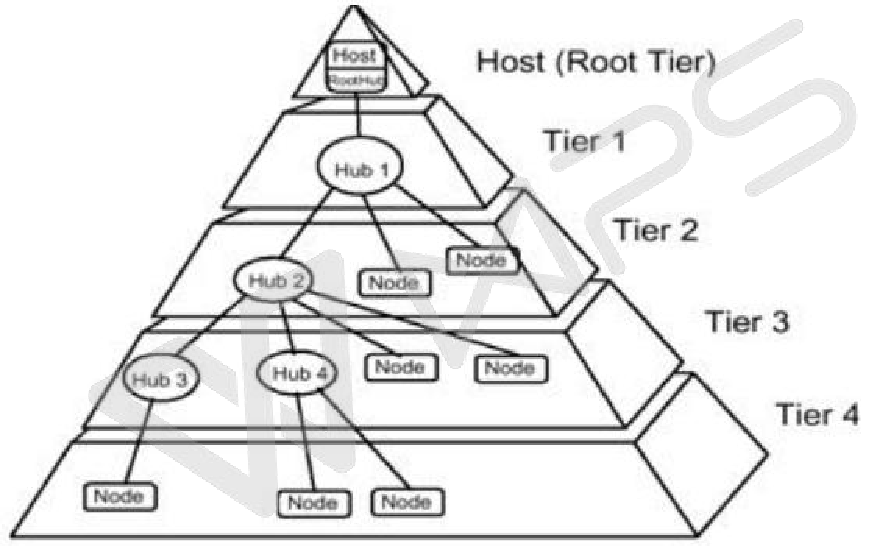
\includegraphics[width=1.0\textwidth]{./graphics/usb-structure.pdf}
\caption{USB总线拓扑结构}\label{fig:USB体系结构}
\end{figure}


USB的体系结构包括三个部分:USB主机(Host)、USB集线器(Hub)、USB设备(Device)。
	
\begin{enumerate}
\item \textbf{USB主机}\\
	USB主机是USB体系中的核心,且系统中只允许一个USB主机存在。USB主机上的USB接口是USB主控制器,其控制着总线上所有USB设备数据通信。对于USB的体系结构而言,其数据的传输都是USB主机端发起的,非主机端(设备端)只能够被动的进行响应。USB主机需要完成的功能包括检测设备的热插拔、管理主机和设备之间的信息(控制和数据)流\cite{李雪红2004USB}\cite{莫宏伟2001USB}。

\item \textbf{USB集线器}\\	
	USB集线器的作用是扩展USB的通讯能力,他可以提供更多的接入口,USB主机上的集线器被称为根集线器,集线器大大的简化了USB的复杂性,而且以很低的价格和易用性提供了设备的健壮性\cite{李雪红2004USB},集线器的最大的连接能力是127。


\item \textbf{USB设备}

	USB设备指的是提供具体功能的而外部USB设备,是相对USB主机而言的,它们受USB主机的控制,只能对主机的请求进行被动响应。USB主机端会通过协议和USB设备通信,对设备进行配置,并给设备提供驱动程序,USB设备通过以下的属性来完成主机的配置要求:
	\begin{itemize}
	\item \textbf{描述符(Descriptor)}\\
	USB协议中定义了一套描述USB设备的功能和属性的固定结构的描述符,包括设备描述符、配置描述符、接口描述符、端点描述符、字符串描述符\cite{张杰2008基于}\cite{边海龙2004USB}除此之外,设备还可以提供自己专用的描述符,分为设备类描述符和供应商自定义描述符,我们使用的USB口转串口设备就不属于一个标准的USB设备,它会为我们提供供应商自定义的描述符,我们之后需要用它来对设备进行识别。
	
	\item \textbf{类(Class)}\\
	USB协议支持许多的外围设备,为了正确的驱动这些设备,USB主机端要为这些设备提供符合USB协议的驱动程序,称为客户端驱动。同时为了避免客户端程序过多,协议通过归纳将设备划分为不同的设备类,把功能相近的设备归为一类,主机端只需要提供类驱动程序便可以驱动大多数的USB设备\cite{李雪红2004USB}。	
	
	\item \textbf{功能(Function)/接口(Interface)}\\
	USB协议中将功能或接口定义为具有某种能力的设备,FUnction是从功能角度来说的,从设备的角度来说,被称为Interface。一个接口负责完成设备的一个特定的功能,并且是可替换的,当USB设备处于可配置状态是能够改变其功能,对于USB设备的每一个接口都必须要有一个接口描述符来描述。
	
	\item \textbf{端点(Endpoint)}\\
	端点是USB设备与USB主机逻辑上的数据传输的通信流的终点,每个设备都拥有一个可独立进行操作的端点集合,且每个端点在使用时都要先初始化其数据传输方向(IN/OUT),即使端点号相同但是传输方向不同的通信点也是不同的端点。端点0被USB规范保留用作设备枚举和配置过程中的数据传输端点,与端点0对应的管道是默认管道,设备的所有端点共享端点0\cite{李雪红2004USB}。
	
	\item \textbf{管道}\\
	管道是设备上的一个端点和主机上的软件的联合体,是一个具有特定数据传输特性(如格式、带宽、方向等)的数据通道,设备和主机间的数据传输要基于管道进行。对USB设备进行配置时就需要建立传输管道,在我们的USB口转串口驱动中会为每一个设备建立两个管道,一个批量输出管道和一个批量输入管道。另外端点0会自动的拥有一个缺省管道。
	\item \textbf{设备地址}\\
	设备地址用于区分USB系统中的一个USB设备,设备地址由主机分配且是唯一的。设备地址共有7位,地址0是缺省地址,在设备初始化的时候使用,理论上系统可以区分127个USB设备,实际中由于USB总线带宽的限制,无法同时支持这么多设备工作\cite{李雪红2004USB}。
	\end{itemize}	
	
\end{enumerate}



\noindent USB规范规定了USB主从设备之间的四种传输方式,每种方式有各自的用途\cite{USB总线接口开发指南}:
\begin{itemize}
\item \hei{控制传输}:控制传输USB传输方式中最重要、最复杂的一种,它适用于少量、对时间和速率无要求的场合,一个USB设备插入主机之后就是使用这种传输方式来读取设备的地址和描述符等信息。所有的设备都会在其0号端点的缺省管道当中支持控制传输\cite{张杰2008基于}。
\item \hei{批量传输}:批量传输有两种最基本的事物类型:BULK\_ IN和BULK\_ OUT,其主要用于处理对数据传输速率不是很高的情况,批量传输使我们的USB口转串口设备所使用的主要传输传输方式,每次有数据需要传输时我们都会构建一个IRP使用批量传输将其传出或传入。
\item \hei{中断传输}:中断传输也有两种基本的事务:IN和OUT,其主要是为那些要快速实现主机和设备的交互,但是数据量很小、对服务时间有要求的情况而准备的。
\item \hei{等时传输}:等时传输也是由基本的IN和OUT两种事务组成,主要用于处理大量、恒速、对时间周期有要求的数据。等时传输只有全速和高速设备才支持,低速设备不支持\cite{张杰2008基于}。
\end{itemize}


	

\section{本章小结}
	本章重点介绍了本次的VxWorks调试通道的整体架构,并介绍了介绍了各个部分的设计方案,最后介绍了在本次的设计当中所需要使用关键技术和所需了解的重要知识,主要包括VxWorks下的驱动开发必须的结构、驱动中所需使用的VxWorks的通信机制、缓冲区技术、USB技术。下面将要讨论VxWorks下的调试通道的详细的设计细节和具体的实际机制。

























